\documentclass[conference]{IEEEtran}
\IEEEoverridecommandlockouts

\usepackage{cite}
\usepackage{amsmath}
\usepackage{newtxmath}
% Times-like text font for XeTeX (Tectonic): TeX Gyre Termes.
\usepackage{fontspec}
\setmainfont{texgyretermes}[Extension=.otf, UprightFont=*-regular,
  BoldFont=*-bold, ItalicFont=*-italic, BoldItalicFont=*-bolditalic]
\usepackage{graphicx}
\usepackage{booktabs}
\usepackage{array}
\usepackage{xcolor}
\usepackage{tikz}
\usetikzlibrary{positioning,arrows.meta,fit,backgrounds}
\usepackage{pgfplots}
\pgfplotsset{compat=1.17}
\usepackage{algorithm}
\usepackage{algpseudocode}
\usepackage{xurl}
\usepackage[hidelinks]{hyperref}

\definecolor{teal}{HTML}{0E7C7B}
\definecolor{burnt}{HTML}{B5531B}
\definecolor{navy}{HTML}{10202B}

\newcolumntype{L}[1]{>{\raggedright\arraybackslash}p{#1}}
\newcommand{\code}[1]{\texttt{#1}}

\begin{document}

\title{An End-to-End MLOps System for Vietnamese License Plate Recognition: From Synthetic Training to Monitored Production Serving}

\author{
\IEEEauthorblockN{Nguyen Dinh Dan, Hoang Xuan Son, Nguyen Hoang Thai, Nguyen Van Vu}
\IEEEauthorblockA{Group 4, DDM501 --- AI in Production: From Models to Systems\\
FPT School of Business and Technology (FSB), Vietnam}
}

\maketitle

\begin{abstract}
Automatic license plate recognition (ALPR) is a mature computer-vision task, yet
deployed recognizers fail silently when lighting, weather or cameras change. This
paper presents an end-to-end machine learning operations (MLOps) system for
Vietnamese license plates that treats the model as one component of a monitored,
reproducible lifecycle. A YOLOv8 detector and a HOG+SVM character classifier are
served through a FastAPI service that always loads the model version tagged
\code{@production} in an MLflow registry. Apache Airflow retrains the model weekly
behind a data-quality gate and a champion/challenger promotion rule; Prometheus,
Grafana and Alertmanager monitor system health and label-free input and
prediction drift through twelve custom metrics and fifteen alert rules; a
continuous-integration pipeline enforces 80\% test coverage and an end-to-end
quality gate. The deployed classifier reaches 92.93\% character accuracy and
93.35\% macro-F1 on a synthetic test set and reads 85.0\% of synthetic plates
exactly, but only 35.7\% (15/42; 95\% CI 23--51\%) of manually labelled real
images. The evaluation and monitoring stack localized this gap to motorbike and
blue plates and to the image-processing path, rejected four weaker retrained
models, and detected a real cold-start latency fault. We describe the design in
enough detail to be reproduced, verify each lifecycle capability with a concrete
scenario, assess the system against the ML Test Score, and report the
engineering failures that the MLOps practices exposed and the limitations that
remain.
\end{abstract}

\begin{IEEEkeywords}
MLOps, license plate recognition, model registry, drift monitoring,
continuous integration, responsible AI
\end{IEEEkeywords}

%==========================================================================
\section{Introduction}
Parking lots, toll stations, residential compounds and gated factories in
Vietnam still record license plates largely by hand. A guard reads the plate,
types it into a logbook or spreadsheet and compares it with the plate at exit.
The process is slow at peak hours, error-prone at night and in rain, and
requires staff around the clock. ALPR is a well-studied answer to this
problem~\cite{du2013alpr,silva2018alpr}, but a recognizer that scores well offline
is not yet a dependable system. Input distributions drift with lighting, weather,
dirt and camera replacement, and in production there are no labels to reveal the
degradation. Sculley \emph{et al.}~\cite{sculley2015debt} showed that the model is
a small part of a real ML system and that most risk lies in data dependencies,
configuration and monitoring; surveys of industrial deployments confirm that
operating a model is harder than training it~\cite{amershi2019se4ml,paleyes2022challenges}.

This project therefore targets the \emph{lifecycle} rather than the strongest
possible model. We ask three research questions:
\begin{itemize}
\item \textbf{RQ1} (engineering): can a small team build a lifecycle in which
data, training, registry, serving, monitoring and retraining are connected by
explicit, automated quality gates, using only open-source components on one
machine?
\item \textbf{RQ2} (evaluation): how large is the gap between the synthetic
benchmark used for training and real Vietnamese plate images, and where in the
pipeline do the errors originate?
\item \textbf{RQ3} (operations): which failures do MLOps practices actually
catch that ordinary testing would not?
\end{itemize}

The contributions are:
\begin{itemize}
\item a containerized system of twelve services covering data validation,
training, experiment tracking, a model registry with alias-based promotion,
serving, monitoring, alerting and scheduled or drift-triggered retraining;
\item a shared champion/challenger rule that promotes a model only above a quality
gate \emph{and} when it is not worse than the serving model, with hot reload and
one-step rollback;
\item label-free drift signals (input brightness, input resolution and the rate of
outputs that match plate grammar) wired into Prometheus alerts, a Grafana
dashboard and an Airflow monitoring DAG, plus a simulation toolkit that
reproduces seven traffic and drift scenarios;
\item an evaluation on 42 manually labelled real images that quantifies the
synthetic-to-real gap and attributes the errors to pipeline stages and plate
groups;
\item an account of six silent failures that the MLOps practices turned into
visible, fixed defects, and a self-assessment against the ML Test
Score~\cite{breck2017mltest}.
\end{itemize}

Section~\ref{sec:related} reviews related work and Section~\ref{sec:problem}
defines the problem. Sections~\ref{sec:arch}--\ref{sec:mlops} describe the
architecture, the ML pipeline and the MLOps lifecycle. Section~\ref{sec:eval}
evaluates model and system, Section~\ref{sec:rai} covers responsible AI, and
Sections~\ref{sec:disc}--\ref{sec:concl} discuss lessons, limitations and future
work. The appendix lists the commands needed to reproduce the results.

%==========================================================================
\section{Related Work}\label{sec:related}
\textit{License plate recognition.} Classical ALPR pipelines detect the plate,
segment characters and classify them~\cite{du2013alpr}. Histograms of oriented
gradients (HOG)~\cite{dalal2005hog} with support vector machines
(SVM)~\cite{cortes1995svm} remain a strong CPU-only baseline for isolated
characters, while single-stage detectors such as YOLO~\cite{redmon2016yolo,
jocher2023yolov8} are the common choice for plate localization. Deep
segmentation-free recognizers such as CRNN~\cite{shi2017crnn} and the
unconstrained-scenario pipeline of Silva and Jung~\cite{silva2018alpr} achieve
higher accuracy but need large labelled real datasets and, usually, a GPU.
Contrast-limited adaptive histogram equalization
(CLAHE)~\cite{zuiderveld1994clahe} is a standard pre-processing step under uneven
lighting. Vietnamese plates add specific difficulties: two-line motorbike plates
with a two-character series and a hyphen, several background colours (white,
yellow, blue) and a restricted alphabet.

\textit{MLOps.} Kreuzberger \emph{et al.}~\cite{kreuzberger2023mlops} define MLOps
as the combination of continuous integration, delivery and training with
experiment tracking, a model registry and monitoring. Google's maturity
model~\cite{google2020mlops} distinguishes manual deployment (level~0), automated
training pipelines (level~1) and automated pipeline delivery (level~2). The ML
Test Score~\cite{breck2017mltest} lists 28 data, model, infrastructure and
monitoring tests needed for production readiness, and MLflow~\cite{zaharia2018mlflow}
is a widely used open-source tracking and registry tool. Amershi \emph{et
al.}~\cite{amershi2019se4ml} and Paleyes \emph{et al.}~\cite{paleyes2022challenges}
report that data management, deployment and monitoring dominate the effort in
practice.

\textit{Drift and responsible AI.} Concept and data drift are surveyed
in~\cite{gama2014drift,lu2019drift}; Rabanser \emph{et al.}~\cite{rabanser2019failing}
argue for detecting shift from unlabelled inputs, which motivates our label-free
signals. SHAP~\cite{lundberg2017shap} and LIME~\cite{ribeiro2016lime} provide global
and local explanations, and model cards~\cite{mitchell2019modelcards} encourage
reporting performance per subgroup.

%==========================================================================
\section{Problem Definition and Requirements}\label{sec:problem}
\subsection{Task and scope}
The system receives a vehicle or plate image through a REST API and returns the
plate string. A Vietnamese plate string $s$ is valid if it consists of a
two-digit province code, a series letter, an optional second series character
and three to five digits, e.g., \code{51F12345} or \code{29AB1234}. The scope is
one- and two-line plates, one plate per still image. Real-time video tracking,
multiple plates per image and foreign plates are out of scope.

\subsection{Stakeholders and use cases}
The primary users are parking and gate operators, who need a plate string per
vehicle within a few seconds; the secondary users are the ML engineers and
operators who maintain the service, who need to know when quality degrades and
how to roll back. Three use cases drive the design: (U1) an entry camera posts a
full scene; (U2) an existing detector posts a pre-cropped plate; (U3) an operator
investigates an alert, inspects the serving model and, if needed, rolls back.

\subsection{Requirements and success metrics}
Table~\ref{tab:req} lists the prioritized requirements with their
implementation status, and Table~\ref{tab:metrics} the success metrics on three
levels: business, model and system. Targets were fixed before the real-image
evaluation, and two of them are not met; we report them as such.

\begin{table}[t]
\centering
\caption{Prioritized requirements and status}
\label{tab:req}
\setlength{\tabcolsep}{4pt}
\begin{tabular}{@{}lL{5.0cm}l@{}}
\toprule
ID & Requirement & Status \\
\midrule
FR1 & Recognize the plate in an uploaded image via REST API & Done \\
FR5 & Monitor system and model through dashboards & Done \\
NFR1 & p95 latency below 3\,s per image & Not met \\
FR2 & Accept full scenes and pre-cropped plates & Done \\
FR3 & Expose health and model information & Done \\
NFR3 & Reproducible containerized deployment & Done \\
FR4 & Track experiments and model versions & Done \\
NFR2 & Alerting on failure and drift & Done \\
NFR4 & CI/CD with quality gates & Done \\
NFR5 & Explainability and fairness analysis & Done \\
\bottomrule
\end{tabular}
\end{table}

\begin{table}[t]
\centering
\caption{Success metrics: targets and measured values}
\label{tab:metrics}
\resizebox{\columnwidth}{!}{%
\begin{tabular}{@{}llll@{}}
\toprule
Level & Metric & Target & Measured \\
\midrule
Business & Exact plate, 42 real images & $>70\%$ & 35.7\% (not met) \\
Business & Throughput, one client & $>10$/min & $\approx$64/min \\
Model & Character accuracy & $>90\%$ & 92.93\% \\
Model & Character macro-F1 & $>90\%$ & 93.35\% \\
Model & Digit/letter accuracy gap & $<10\%$ & 1.0\% \\
System & p95 latency, real images & $<3$\,s & $\approx$4.1\,s (not met) \\
System & Test coverage & $>80\%$ & 81.8\% \\
System & Time to alert, API down & $<5$\,min & $\approx$75\,s \\
\bottomrule
\end{tabular}}
\end{table}

%==========================================================================
\section{System Architecture}\label{sec:arch}
\subsection{Components}
Fig.~\ref{fig:arch} shows the system and Table~\ref{tab:services} its services.
Twelve containers run on one Docker Compose network: ten long-running services,
each with a health check, and two one-shot initializers (MinIO bucket creation
and Airflow database migration). A thirteenth service, the \code{trainer}, is
started on demand through a Compose profile. Each service has a single
responsibility, so a failure is contained: if MLflow is unavailable the API keeps
serving its last loaded model, and if the API is down Prometheus still records
\code{up=0} and raises an alert.

\begin{figure*}[t]
\centering
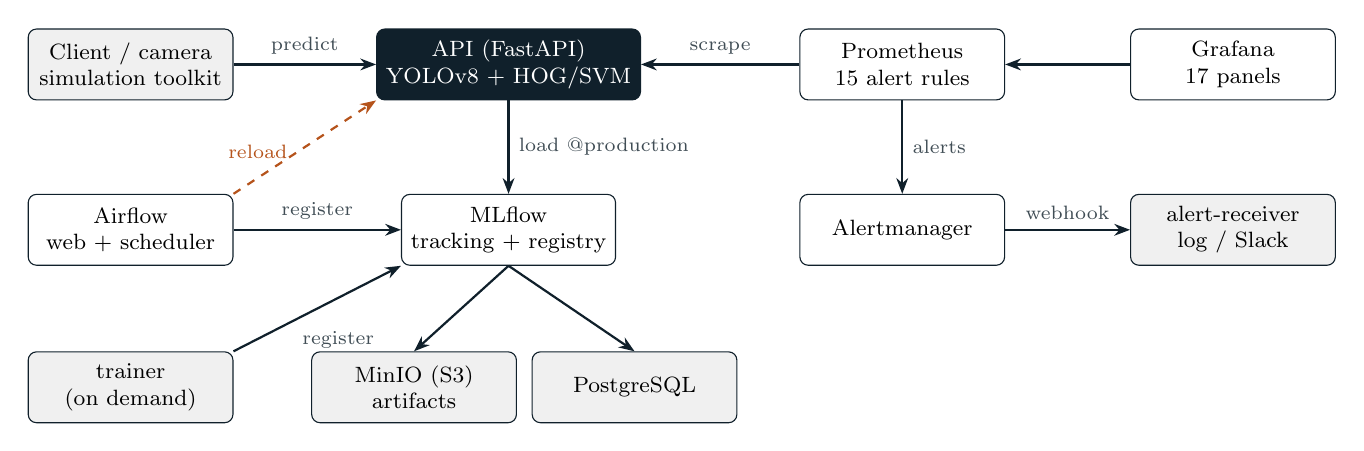
\begin{tikzpicture}[
  font=\footnotesize,
  box/.style={draw=navy, rounded corners=3pt, align=center, minimum height=9mm, minimum width=26mm, fill=white},
  core/.style={box, fill=navy, text=white},
  store/.style={box, fill=gray!12},
  arr/.style={-{Stealth[length=2mm]}, thick, navy},
  lbl/.style={font=\scriptsize, text=navy!80}
]
% row 1: request path and observability
\node[store] (client) at (0,0) {Client / camera\\simulation toolkit};
\node[core]  (api)    at (4.8,0) {API (FastAPI)\\YOLOv8 + HOG/SVM};
\node[box]   (prom)   at (9.8,0) {Prometheus\\15 alert rules};
\node[box]   (graf)   at (14.0,0) {Grafana\\17 panels};
% row 2: lifecycle and alerting
\node[box]   (airflow) at (0,-2.1) {Airflow\\web + scheduler};
\node[box]   (mlflow)  at (4.8,-2.1) {MLflow\\tracking + registry};
\node[box]   (am)      at (9.8,-2.1) {Alertmanager};
\node[store] (recv)    at (14.0,-2.1) {alert-receiver\\log / Slack};
% row 3: storage and on-demand training
\node[store] (trainer) at (0,-4.1) {trainer\\(on demand)};
\node[store] (minio)   at (3.6,-4.1) {MinIO (S3)\\artifacts};
\node[store] (pg)      at (6.4,-4.1) {PostgreSQL};

\draw[arr] (client.east) -- node[lbl, above]{predict} (api.west);
\draw[arr] (prom.west) -- node[lbl, above]{scrape} (api.east);
\draw[arr] (graf.west) -- (prom.east);
\draw[arr] (prom.south) -- node[lbl, right]{alerts} (am.north);
\draw[arr] (am.east) -- node[lbl, above]{webhook} (recv.west);
\draw[arr] (api.south) -- node[lbl, right]{load @production} (mlflow.north);
\draw[arr] (airflow.east) -- node[lbl, above]{register} (mlflow.west);
\draw[arr, dashed, burnt] (airflow.north east) -- node[lbl, left, text=burnt, pos=0.45]{reload} (api.south west);
\draw[arr] (mlflow.south) -- (minio.north);
\draw[arr] (mlflow.south) -- (pg.north);
\draw[arr] (trainer.north east) -- node[lbl, below right, pos=0.35]{register} (mlflow.south west);
\end{tikzpicture}
\caption{System architecture. Solid arrows are data or control flow; the dashed
arrow is the hot reload issued after a promotion. The monitoring DAG in Airflow
also queries Prometheus (not drawn).}
\label{fig:arch}
\end{figure*}

\begin{table}[t]
\centering
\caption{Services of the Docker Compose stack}
\label{tab:services}
\setlength{\tabcolsep}{3pt}
\footnotesize
\begin{tabular}{@{}lrL{4.4cm}@{}}
\toprule
Service & Port & Role \\
\midrule
\code{postgres} & 5432 & Metadata store for MLflow and Airflow \\
\code{minio} & 9000/1 & S3-compatible artifact store \\
\code{minio-init} & --- & One-shot: creates the artifact bucket \\
\code{mlflow} & 5000 & Tracking server, registry, artifact proxy \\
\code{api} & 8000 & FastAPI inference service \\
\code{trainer} & --- & On-demand training job (profile \code{train}) \\
\code{prometheus} & 9090 & Metrics scraping and alert rules \\
\code{alertmanager} & 9093 & Alert grouping, routing, inhibition \\
\code{alert-receiver} & 9094 & Webhook sink, log, optional Slack \\
\code{grafana} & 3000 & Provisioned dashboard \\
\code{airflow-init} & --- & One-shot: database migration, admin user \\
\code{airflow-web.} & 8080 & Airflow UI and REST API \\
\code{airflow-sched.} & --- & DAG scheduling (LocalExecutor) \\
\bottomrule
\end{tabular}
\end{table}

\subsection{Request flow}
A prediction request passes through six steps: (1) a middleware applies a
sliding-window rate limit per client IP and answers HTTP~429 with a
\code{Retry-After} header when it is exceeded; (2) the upload size is checked
against a 10\,MB limit (HTTP~413); (3) the image is decoded in memory, and
invalid images are rejected with HTTP~400; (4) the input brightness and width are
recorded as drift metrics; (5) recognition runs in a thread pool so that
\code{/health} and \code{/metrics} stay responsive during long inferences; and
(6) prediction count, latency, character count, detection confidence and the
outcome of the plate-grammar check are recorded before the JSON response is
returned. The response carries the corrected plate text, the raw classifier
output, the plate type, the number of characters, the detection confidence, a
plate-format score, the latency and a timestamp.

\subsection{Technology choices}
Docker Compose was preferred to Kubernetes because the system runs on a single
machine for this course; the API is stateless and loads its model from the
registry, so replicas behind a load balancer need no code change. HOG+SVM was
preferred to a deep OCR network because it runs on CPU, yields a small model,
trains in seconds and can be explained with SHAP and LIME; the OCR stage is
isolated behind one interface, so a stronger recognizer can replace it without
touching the MLOps layer. MinIO provides S3-compatible artifact storage proxied by
MLflow, so only the MLflow server holds storage credentials. Airflow was chosen
over cron because it records every run, retries failed tasks and exposes a REST
API that the monitoring DAG uses to trigger retraining.

%==========================================================================
\section{ML Pipeline}\label{sec:ml}
\subsection{Inference stages}
Each request runs seven stages.

\textit{(1) Enhancement.} The image is converted to grayscale and enhanced with
CLAHE~\cite{zuiderveld1994clahe} (clip limit 2.0, $8\times8$ tiles) followed by a
bilateral filter ($d=9$, $\sigma=75$) that removes noise while keeping character
edges.

\textit{(2) Detection.} A YOLOv8n model~\cite{jocher2023yolov8} fine-tuned on
plates returns the plate box with a confidence threshold of 0.25. When the
weights are absent or detect nothing, a fallback finds rectangular contours whose
aspect ratio matches Vietnamese plates. Requests may set
\code{assume\_plate\_crop} to skip detection for pre-cropped input (use case U2).

\textit{(3) Rectification.} The crop is rectified by a perspective transform,
deskewed by the dominant text angle, and both $0^\circ$ and $180^\circ$
orientations are evaluated.

\textit{(4) Plate type.} The aspect ratio $\rho=w/h$ decides between a one-line
($\rho>2.5$) and a two-line plate; the type controls how characters are split into
rows.

\textit{(5) Segmentation.} For several enhanced variants of the crop
(CLAHE with clip 3.0 and $4\times4$ tiles, bilateral filter $d=5$, $\sigma=45$),
Otsu binarization is applied in normal and inverted polarity. Connected
components are filtered by area, height ($10$--$82\%$ of the plate height),
width and aspect ratio ($<1.9$); each candidate binarization is scored by the
number of plausible components, their fill ratio and penalties for huge or
border-touching blobs. Characters are sorted by row and column and normalized to
$32\times32$ pixels.

\textit{(6) Classification.} HOG features are computed with $4\times4$-pixel cells,
$2\times2$-cell blocks and 9 orientation bins. A $32\times32$ character has
$8\times8$ cells and $7\times7$ overlapping blocks, so the descriptor has
\begin{equation}
D = 7 \cdot 7 \cdot (2 \cdot 2 \cdot 9) = 1764
\label{eq:hogdim}
\end{equation}
dimensions (the alternative $8\times8$-pixel cells give $3\cdot3\cdot36=324$).
Features are standardized, $z=(x-\mu)/\sigma$, and classified by an SVM with the
radial basis function kernel,
\begin{equation}
f(\mathbf{z}) = \sum_{i} \alpha_i y_i \exp\!\bigl(-\gamma \lVert \mathbf{z}_i - \mathbf{z} \rVert^2\bigr) + b,
\label{eq:svm}
\end{equation}
combined one-versus-one over 31 classes: the ten digits and the 21 letters used
on Vietnamese plates (I, J, O, Q and W are excluded).

\textit{(7) Plate grammar.} Each position has a character type: positions 1--2
must be digits, position 3 a letter and the tail digits. The classifier's scores
are first constrained to the allowed classes per position; remaining confusions
are corrected with fixed maps (Table~\ref{tab:grammar}). The final text is matched
against the valid-plate pattern, and a plate-format score (0--20) summarizes how
well the candidate fits. Among all crop variants, orientations and binarizations,
the candidate with the highest score is returned; evaluation stops early when a
valid plate scores at least 12, and a wider fallback search runs when the best
score is below 10.

\begin{table}[t]
\centering
\caption{Grammar-based correction maps}
\label{tab:grammar}
\setlength{\tabcolsep}{4pt}
\begin{tabular}{@{}lL{5.3cm}@{}}
\toprule
Expected & Correction \\
\midrule
Digit & B$\to$8, G$\to$6, I/L/T$\to$1, O$\to$0, S$\to$5, Z$\to$2 \\
Letter & 0$\to$G, 1$\to$L, 4$\to$A, 5$\to$S, 6$\to$G, 8$\to$B \\
\bottomrule
\end{tabular}
\end{table}

\subsection{Training data}
Real labelled character crops were not available, so the classifier is trained on
synthetic characters. For each of the 31 classes the generator renders 250 clean
glyphs and 400 ``plate-style'' glyphs from TrueType fonts. Plate-style glyphs are
perturbed with Gaussian blur, erosion or dilation, additive noise and random
thresholding (thresholds 35--95), which imitates low-resolution, over- or
under-exposed plates. This gives $31 \times 650 = 20{,}150$ samples, split 80/20
with stratification (16{,}120 training and 4{,}030 test characters). Generation is
deterministic: seeds are fixed and the same fonts are installed in every
container image, so two runs on different machines produce identical data.

Before training, a data gate computes a validation report (sample count, class
count, minimum and maximum samples per class, imbalance ratio, presence of NaN,
pixel range) and stops the pipeline with a non-retryable failure on NaN values,
pixels outside $[0,255]$ or fewer than 31 classes.

\subsection{Real-image evaluation set}
To measure real performance, the team labelled the plate text of 50 sample
images from a public plate-detection dataset. Eight images were unreadable even
for a human (blur, occlusion, extreme angle) and were excluded and listed
separately, leaving 42 labelled images. Each label records a confidence level, the
vehicle type (car or motorbike), the line count and the plate colour, so the
results can be broken down by group. Ground-truth plate boxes from the dataset
were also cropped, which lets us run the OCR stage alone and separate detection
errors from recognition errors.

\subsection{Evaluation metrics}
Character accuracy is the share of correctly classified test characters. Macro-F1
averages the per-class F1 score with equal weight per class,
\begin{equation}
\text{F1}_{\text{macro}} = \frac{1}{K}\sum_{k=1}^{K} \frac{2 P_k R_k}{P_k + R_k},
\label{eq:f1}
\end{equation}
where $P_k$ and $R_k$ are precision and recall of class $k$ and $K=31$; it
penalizes weak rare classes that accuracy would hide. Exact-plate accuracy counts
a plate as correct only if every character is correct, which is the business
metric. For small samples we report the Wilson score interval~\cite{wilson1927}
for a proportion $\hat p$ over $n$ trials,
\begin{equation}
\frac{\hat p + \frac{z^2}{2n} \pm z\sqrt{\frac{\hat p(1-\hat p)}{n} + \frac{z^2}{4n^2}}}{1+\frac{z^2}{n}},
\label{eq:wilson}
\end{equation}
with $z=1.96$ for 95\% confidence.

\subsection{Experiments and model selection}
Table~\ref{tab:grid} compares sixteen feature/classifier combinations on a fixed
synthetic split using scikit-learn~\cite{pedregosa2011sklearn}: four feature
extractors (raw pixels, Haar wavelets, HOG-324 and HOG-1764) and four classifiers
(SVM, logistic regression, random forest and $k$-nearest neighbours). HOG
features dominate raw pixels and wavelets, and the SVM is the strongest
classifier for the 324-dimensional HOG variant. Five-fold cross-validation of the
top configuration gives a macro-F1 of $0.936\pm0.057$. Logistic regression is
competitive in accuracy but slower to fit by two to three orders of magnitude,
which matters for weekly retraining.

\begin{table}[t]
\centering
\caption{Feature $\times$ classifier comparison (synthetic split)}
\label{tab:grid}
\setlength{\tabcolsep}{4pt}
\begin{tabular}{@{}llrrr@{}}
\toprule
Feature & Classifier & Accuracy & Macro-F1 & Fit (s) \\
\midrule
HOG-324 & SVM & 94.12 & 94.15 & 0.6 \\
HOG-324 & Logistic & 93.43 & 93.44 & 82.3 \\
HOG-1764 & Random forest & 92.74 & 92.79 & 1.9 \\
HOG-324 & Random forest & 92.51 & 92.57 & 1.4 \\
HOG-1764 & Logistic & 92.51 & 92.52 & 518.4 \\
HOG-1764 & SVM (untuned) & 89.63 & 90.18 & 5.3 \\
HOG-324 & KNN & 89.98 & 90.13 & 0.0 \\
Wavelet & Random forest & 89.06 & 89.11 & 1.0 \\
Raw & Random forest & 88.71 & 88.75 & 1.1 \\
Raw & SVM & 88.48 & 88.63 & 2.3 \\
Raw & Logistic & 88.02 & 88.05 & 363.6 \\
HOG-1764 & KNN & 87.79 & 87.96 & 0.0 \\
Wavelet & Logistic & 86.06 & 86.14 & 75.8 \\
Wavelet & SVM & 85.83 & 85.91 & 0.7 \\
Raw & KNN & 83.76 & 83.97 & 0.0 \\
Wavelet & KNN & 79.49 & 79.78 & 0.0 \\
\bottomrule
\end{tabular}
\end{table}

The two finalists were retrained on the full data (Table~\ref{tab:final}). The
1764-dimensional model was tuned with three-fold grid search over $C$ and
$\gamma$ (best $C=5$, $\gamma=\text{auto}=1/D$, CV macro-F1 0.921). Although
HOG-324 is better per character, HOG-1764 reads more \emph{whole plates} correctly
on a 60-plate synthetic benchmark. The finer cells keep stroke details that
distinguish confusable pairs within a plate, while HOG-324 wins on isolated
glyphs. Because the business objective is the full plate, HOG-1764 was deployed.
This decision illustrates why the model metric alone should not drive promotion.

\begin{table}[t]
\centering
\caption{Finalists trained on the full synthetic set}
\label{tab:final}
\resizebox{\columnwidth}{!}{%
\begin{tabular}{@{}lrr@{}}
\toprule
Metric & HOG-1764 (deployed) & HOG-324 \\
\midrule
Character accuracy (4{,}030 chars) & 92.93\% & 96.90\% \\
Character macro-F1 & 93.35\% & --- \\
Exact plate, 60 synthetic plates & \textbf{85.0\%} & 81.7\% \\
End-to-end character accuracy & \textbf{96.4\%} & 93.6\% \\
Exact plate with YOLO detection & 83.3\% & --- \\
\bottomrule
\end{tabular}}
\end{table}

%==========================================================================
\section{MLOps Lifecycle}\label{sec:mlops}
\subsection{Experiment tracking}
Every training run, manual or orchestrated, logs to MLflow: parameters
(feature method, classifier, hyper-parameters, sample counts, test size, feature
dimension), metrics (accuracy, macro-F1, cross-validation mean and standard
deviation), tags (trigger reason: \code{scheduled}, \code{manual} or
\code{drift}) and artifacts (classification report, confusion matrix and a
metadata file). Run metadata lives in PostgreSQL and artifacts in MinIO, so the
history survives container restarts.

\subsection{Model registry}
Each model is registered as a single scikit-learn
\code{Pipeline(scaler $\rightarrow$ SVM)} under the registered name
\code{lpr-ocr-classifier}, together with metadata
(feature method, feature dimension, class list, scikit-learn version). Packaging
scaler and classifier together makes training--serving skew in feature scaling
impossible, and the metadata lets the API fail fast if the model expects a
feature dimension the code does not produce. Serving resolves the alias
\code{@production}; MLflow stages are deprecated in favour of aliases. Because the
MLflow~2.17 \code{get\_model\_info} call rejects alias URIs, the shared registry
module first resolves the alias to a concrete version.

Promotion follows one shared rule, implemented once and used by both the Airflow
DAG and manual training:
\begin{equation}
\text{promote} \iff a \ge a_{\min} \;\wedge\; \bigl(a^{*} = \varnothing \,\vee\, a \ge a^{*}\bigr),
\label{eq:promote}
\end{equation}
where $a$ is the challenger accuracy, $a_{\min}=0.90$ and $a^{*}$ is the accuracy
logged by the run behind \code{@production}. Algorithm~\ref{alg:promote} shows the
full procedure. Rollback is a single alias change followed by an authenticated
\code{POST /model/reload}; no container restart is needed, and the previous
version remains in the registry.

\begin{algorithm}[t]
\caption{Champion/challenger registration and promotion}
\label{alg:promote}
\begin{algorithmic}[1]
\Require trained pipeline $m$, test accuracy $a$, metadata $\mu$
\State $v \gets$ \Call{RegisterVersion}{$m$, $\mu$} \Comment{always registered}
\State $a^{*} \gets$ \Call{ChampionAccuracy}{\code{@production}}
\If{$a < a_{\min}$}
  \State tag $v$ as rejected (gate); \Return
\ElsIf{$a^{*} \neq \varnothing$ \textbf{and} $a < a^{*}$}
  \State tag $v$ as rejected (champion); \Return
\EndIf
\State \Call{SetAlias}{\code{production}, $v$}
\State \Call{Post}{\code{/model/reload}, admin token} \Comment{hot reload}
\end{algorithmic}
\end{algorithm}

\subsection{Orchestration}
Two Airflow DAGs run on the LocalExecutor with PostgreSQL as metadata database.
Table~\ref{tab:dags} lists their tasks.
\code{lpr\_training\_pipeline} runs weekly and is unpaused at creation, so
scheduled retraining starts without manual action. Tasks pass small metadata
dictionaries through XCom and large arrays through a per-run directory. Each
task retries twice with a delay, but quality-gate violations raise a
non-retryable failure so that bad data is not retried into a model.
\code{lpr\_monitoring\_pipeline} runs every 15 minutes. It checks API health,
verifies that the version served by the API equals the version behind
\code{@production} (detecting a missed reload), sends a canary image with a
known plate, evaluates PromQL thresholds (Table~\ref{tab:thresholds}) and writes
a JSON report. When drift is detected and \code{AUTO\_RETRAIN\_ON\_DRIFT} is
enabled, a branch triggers the training DAG with the reason \code{drift}.
Statistical checks are skipped when fewer than 20 predictions arrived in the
window, because a p95 over three requests is noise.

\begin{table}[t]
\centering
\caption{Airflow DAG tasks}
\label{tab:dags}
\setlength{\tabcolsep}{3pt}
\footnotesize
\begin{tabular}{@{}lL{4.8cm}@{}}
\toprule
Task & Purpose \\
\midrule
\multicolumn{2}{@{}l}{\textit{lpr\_training\_pipeline (@weekly)}} \\
\code{generate\_data} & Render 20{,}150 synthetic characters (fixed seed) \\
\code{validate\_data} & Data gate: NaN, pixel range, 31 classes, imbalance \\
\code{extract\_features} & HOG-1764 descriptors \\
\code{train} & Standardize, 3-fold CV (macro-F1), fit SVM, log to MLflow \\
\code{evaluate} & Accuracy, macro-F1, report, confusion matrix \\
\code{register\_model} & Register version, apply rule~\eqref{eq:promote} \\
\code{reload\_api} & Hot reload, only after a promotion \\
\midrule
\multicolumn{2}{@{}l}{\textit{lpr\_monitoring\_pipeline (every 15 min)}} \\
\code{check\_api\_health} & \code{/health} and model loaded \\
\code{check\_model\_consistency} & Served version $=$ \code{@production} \\
\code{canary\_prediction} & Known image returns expected plate \\
\code{query\_prometheus} & Success rate, p95, errors, drift ratios \\
\code{evaluate\_health\_and\_drift} & Compare with thresholds \\
\code{write\_monitoring\_report} & JSON report per run \\
\code{branch\_on\_drift} & Trigger retraining or no action \\
\code{fail\_if\_unhealthy} & Make an unhealthy run visible as failed \\
\bottomrule
\end{tabular}
\end{table}

\begin{table}[t]
\centering
\caption{Monitoring DAG thresholds (environment-configurable)}
\label{tab:thresholds}
\setlength{\tabcolsep}{4pt}
\begin{tabular}{@{}lr@{}}
\toprule
Check & Threshold \\
\midrule
Recognition success rate & $\ge 0.5$ \\
p95 prediction latency & $\le 3.0$\,s \\
Error rate & $\le 0.1$/s \\
Brightness drift ratio $r_b$ & $\le 0.3$ \\
Width drift ratio $r_w$ & $\le 0.5$ \\
Minimum predictions for statistical checks & 20 \\
\bottomrule
\end{tabular}
\end{table}

\subsection{Serving}
Table~\ref{tab:endpoints} lists the endpoints. The OpenAPI specification
documents every request and response field with examples and every error code
with a typed error body. Security and robustness measures are: uploads limited to
10\,MB; a limit of 60 requests per minute per client; a token, compared in
constant time, for the reload endpoint; error responses that never contain stack
traces or internal paths; a non-root user in a multi-stage image; and a check that
refuses to load a Git LFS pointer file in place of model weights. A warm-up
inference at start-up and after every reload moves the one-off initialization of
the detector and feature extractor off the request path. If MLflow cannot be
reached, the API falls back to the local model files and reports
\code{model\_source: local} in \code{/model/info}, which makes the degraded mode
visible.

\begin{table}[t]
\centering
\caption{REST endpoints}
\label{tab:endpoints}
\setlength{\tabcolsep}{3pt}
\footnotesize
\begin{tabular}{@{}llL{4.1cm}@{}}
\toprule
Method & Path & Purpose \\
\midrule
GET & \code{/} & Service information and links \\
GET & \code{/health} & Liveness and model readiness \\
GET & \code{/model/info} & Version, source, feature method, metrics \\
POST & \code{/predict} & Multipart image, optional \code{assume\_plate\_crop} \\
POST & \code{/predict/base64} & Base64-encoded JPEG or PNG \\
POST & \code{/model/reload} & Load current \code{@production} (\code{X-Admin-Token}) \\
GET & \code{/metrics} & Prometheus exposition format \\
\bottomrule
\end{tabular}
\end{table}

\subsection{Monitoring}
The API exports twelve custom metrics (Table~\ref{tab:prom}), scraped by
Prometheus every 10\,s. Because production traffic is unlabelled, model quality is
observed through proxies. \emph{Data drift} is measured on the input brightness
$b$ and width $w$ by comparing a recent window with a baseline,
\begin{equation}
r_b = \left|1 - \frac{\bar b_{1\,\mathrm{h}}}{\bar b_{7\,\mathrm{d}}}\right|,
\qquad r_w = \left|1 - \frac{\bar w_{1\,\mathrm{h}}}{\bar w_{7\,\mathrm{d}}}\right|,
\label{eq:drift}
\end{equation}
where each mean is computed in PromQL as the ratio of the histogram's
\code{\_sum} and \code{\_count} rates. A night-time camera lowers $\bar b$; a camera
replacement changes $\bar w$. \emph{Prediction drift} is measured by the share of
outputs that match the plate grammar,
\begin{equation}
s = \frac{N_{\text{valid}}}{N_{\text{valid}} + N_{\text{invalid}}},
\label{eq:success}
\end{equation}
which falls when inputs move away from the training distribution even though no
label is available. The Grafana dashboard provisions 17 panels in three rows:
service health (request rate, latency percentiles and heatmap, errors, status
codes, uptime, model information), model behaviour (predictions by plate type,
detection confidence, characters per plate) and drift (success rate, brightness
and width against their baselines, in both production and fast windows).

\begin{table}[t]
\centering
\caption{Custom Prometheus metrics exported by the API}
\label{tab:prom}
\setlength{\tabcolsep}{3pt}
\footnotesize
\begin{tabular}{@{}lL{3.3cm}@{}}
\toprule
Metric (type) & Meaning \\
\midrule
\code{api\_requests\_total} (C) & Requests by method, endpoint, status \\
\code{api\_request\_latency\_seconds} (H) & End-to-end request latency \\
\code{model\_predictions\_total} (C) & Predictions by plate type \\
\code{model\_prediction\_latency\_seconds} (H) & Inference latency \\
\code{model\_prediction\_errors\_total} (C) & Errors by type (incl. rate limit) \\
\code{model\_info} (G) & Loaded version and source \\
\code{plate\_char\_count} (H) & Characters per plate \\
\code{detection\_confidence} (H) & YOLO confidence \\
\code{plate\_recognition\_result\_total} (C) & Valid vs.\ invalid plate format \\
\code{plate\_format\_score} (H) & Grammar fit score, 0--20 \\
\code{input\_image\_brightness} (H) & Mean grayscale brightness \\
\code{input\_image\_width\_pixels} (H) & Input width \\
\bottomrule
\multicolumn{2}{@{}l}{\scriptsize C: counter, H: histogram, G: gauge.}
\end{tabular}
\end{table}

\subsection{Alerting}
Table~\ref{tab:alerts} lists the fifteen alert rules in five groups. Each rule has
a \code{for} duration so that a single slow request does not page anyone. The
drift rules come in two variants: the production rules compare one hour with
seven days, while the fast rules compare five minutes with one hour so that a
live simulation can fire them during a demonstration. The \code{NoPredictions}
rule sums over plate types, because a plate type that simply did not occur would
otherwise fire the alert while traffic flows.

Alertmanager groups notifications by alert name and severity. Critical alerts
are sent after 10\,s and repeated hourly; informational alerts are batched. An
inhibition rule suppresses warning and informational alerts while
\code{APIDown} fires, because every API metric is meaningless then. All
notifications go to a webhook receiver that logs them, keeps the last 50 in a
queryable endpoint, appends them to a JSON-lines file and optionally forwards
them to Slack.

\begin{table*}[t]
\centering
\caption{Prometheus alert rules}
\label{tab:alerts}
\setlength{\tabcolsep}{4pt}
\footnotesize
\begin{tabular}{@{}llL{8.2cm}lr@{}}
\toprule
Group & Alert & Condition & Severity & For \\
\midrule
api & \code{APIHighErrorRate} & prediction errors $>0.1$/s over 5\,min & warning & 2\,m \\
api & \code{APIHighLatency} & p95 request latency $>5$\,s over 5\,min & warning & 3\,m \\
api & \code{APIDown} & scrape target \code{lpr-api} down & critical & 1\,m \\
model & \code{HighPredictionLatency} & p95 inference latency $>3$\,s & warning & 5\,m \\
model & \code{LowCharacterDetection} & median characters per plate $<5$ & warning & 10\,m \\
model & \code{LowDetectionConfidence} & median YOLO confidence $<0.5$ & warning & 10\,m \\
model & \code{NoPredictions} & total prediction rate over 15\,min $=0$ & info & 30\,m \\
drift & \code{LowRecognitionSuccessRate} & valid-format share $s<0.5$ over 30\,min & warning & 15\,m \\
drift & \code{InputBrightnessDrift} & $r_b>0.3$ (1\,h vs.\ 7\,d) & warning & 30\,m \\
drift & \code{InputResolutionDrift} & $r_w>0.5$ (1\,h vs.\ 7\,d) & warning & 30\,m \\
drift (fast) & \code{InputBrightnessDriftFast} & $r_b>0.3$ (5\,min vs.\ 1\,h) & warning & 2\,m \\
drift (fast) & \code{InputResolutionDriftFast} & $r_w>0.5$ (5\,min vs.\ 1\,h) & warning & 2\,m \\
drift (fast) & \code{LowRecognitionSuccessRateFast} & $s<0.5$ over 5\,min with traffic & warning & 2\,m \\
drift (fast) & \code{RateLimitBurst} & more than 5 HTTP~429 responses in 2\,min & warning & --- \\
system & \code{PrometheusTargetDown} & any scrape target down & critical & 2\,m \\
\bottomrule
\end{tabular}
\end{table*}

\subsection{Simulation toolkit}
To exercise monitoring without a real camera, a simulation toolkit replays images
against the API under seven scenarios: normal traffic, nightfall (gradual
darkening), camera swap (resolution change), mixed weather (motion blur, noise, JPEG compression, occlusion),
prediction drift (non-plate images), a rate-limit spike and malformed inputs.
Drift is produced by deterministic image transforms, so each scenario has a known
expected alert. The toolkit has its own unit tests.

\subsection{Testing and continuous integration}
The suite contains 149 tests in five categories (Table~\ref{tab:tests}) and covers
81.8\% of \code{src/} and \code{api/}. Tests use small fixtures and mocks for
MLflow and Prometheus, so they run without the Docker stack.

GitHub Actions runs three dependent jobs on every push and pull request
(Table~\ref{tab:ci}). The end-to-end benchmark is a \emph{model} gate inside CI: a
change to pre-processing or segmentation that lowers plate accuracy on the
synthetic benchmark fails the build even if every unit test passes. A separate
manual workflow builds and pushes images to the GitHub Container Registry.
Model binaries are stored with Git LFS and cached in CI to save bandwidth.

\begin{table}[t]
\centering
\caption{Test suite by category}
\label{tab:tests}
\setlength{\tabcolsep}{3pt}
\footnotesize
\begin{tabular}{@{}lL{4.6cm}@{}}
\toprule
Category & What is tested \\
\midrule
Unit & Pre-processing, features, classifier, detection, pipeline, grammar, registry module, crop script \\
Integration & All endpoints, auth, size and rate limits, metrics, MLflow fallback, error bodies \\
Data quality & Synthetic data schema, value ranges, class coverage and balance \\
Model validation & Accuracy and macro-F1 thresholds, robustness to noisy inputs \\
Operations & Monitoring DAG logic, alert receiver, simulation transforms and simulator \\
End-to-end & Full pipeline on labelled synthetic plates \\
\bottomrule
\end{tabular}
\end{table}

\begin{table}[t]
\centering
\caption{Continuous integration jobs}
\label{tab:ci}
\setlength{\tabcolsep}{3pt}
\footnotesize
\begin{tabular}{@{}lL{5.2cm}@{}}
\toprule
Job & Steps and gates \\
\midrule
\code{lint} & ruff and black on all Python packages, DAGs and tests \\
\code{test} & pytest with coverage gate 80\%; E2E benchmark gate: character accuracy $\ge85\%$, exact plate $\ge50\%$; reports uploaded as artifacts \\
\code{docker-build} & Build API, MLflow, Airflow and trainer images \\
\bottomrule
\end{tabular}
\end{table}

\subsection{Reproducibility}
Reproducibility is enforced at four levels. \emph{Code}: dependencies are pinned
to exact versions (e.g., scikit-learn 1.5.2, scikit-image 0.24.0, NumPy 1.26.4),
the same versions are used in the trainer and the API, and the version is stored
in the model metadata. \emph{Data}: synthetic data is generated from fixed seeds
and fonts, and the real-image labels are versioned as CSV files with an explicit
list of excluded images. \emph{Models}: every model is an immutable registry
version with its run, parameters and artifacts. \emph{Environment}: the whole
stack is described by one Compose file and a \code{.env.example}; secrets are
never committed.

%==========================================================================
\section{Evaluation}\label{sec:eval}
\subsection{Recognition accuracy (RQ2)}
Fig.~\ref{fig:gap} contrasts the synthetic benchmark with the real images. On the
42 real images the full pipeline reads 15 plates exactly (35.7\%; 95\% Wilson
interval~\eqref{eq:wilson} 23--51\%) with 63.2\% character accuracy.
Table~\ref{tab:groups} breaks the result down. Two-line car plates fare best;
motorbike plates (two-character series and a hyphen on the top line) and blue
plates with white text fail most. The blue-plate failure is a polarity problem:
the segmentation is tuned for dark text on a light background.

Feeding ground-truth plate crops raises character accuracy from 63.2\% to
81.0\% (exact plate 42.9\%). Roughly half of the character errors therefore
originate in detection crops, rectification and deskew rather than in the
classifier, which tells us where to invest next. Images from the detector's
training and validation splits score similarly (37.0\% vs.\ 33.3\%), suggesting
no strong detector overfitting on this sample.

\begin{figure}[t]
\centering
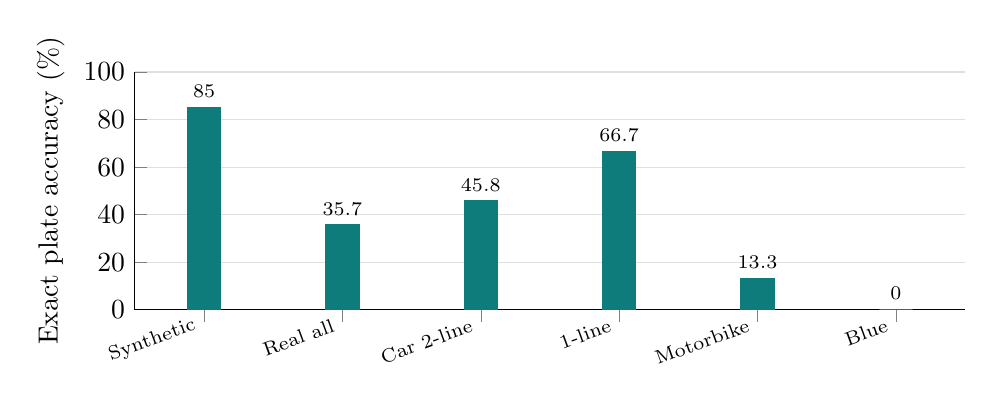
\begin{tikzpicture}
\begin{axis}[
  ybar, width=\columnwidth, height=4.6cm, bar width=12pt,
  ymin=0, ymax=100, ylabel={Exact plate accuracy (\%)},
  symbolic x coords={Synthetic,Real all,Car 2-line,1-line,Motorbike,Blue},
  xtick=data, x tick label style={font=\scriptsize, rotate=20, anchor=east},
  nodes near coords, nodes near coords style={font=\scriptsize},
  every node near coord/.append style={/pgf/number format/fixed,/pgf/number format/precision=1},
  axis lines*=left, ymajorgrids, grid style={gray!25},
]
\addplot[fill=teal, draw=teal] coordinates {(Synthetic,85.0) (Real all,35.7) (Car 2-line,45.8) (1-line,66.7) (Motorbike,13.3) (Blue,0)};
\end{axis}
\end{tikzpicture}
\caption{Synthetic-to-real gap and per-group exact plate accuracy on real images
(1-line and blue groups contain only 3 and 2 images).}
\label{fig:gap}
\end{figure}

\begin{table}[t]
\centering
\caption{Real-image results by group (full pipeline)}
\label{tab:groups}
\begin{tabular}{@{}lrr@{}}
\toprule
Group & Exact plate & Share \\
\midrule
All images & 15/42 & 35.7\% \\
Two-line car plates & 11/24 & 45.8\% \\
Motorbike plates & 2/15 & 13.3\% \\
One-line plates & 2/3 & --- \\
Yellow plates & 4/8 & 50.0\% \\
White plates & 11/32 & 34.4\% \\
Blue plates & 0/2 & --- \\
Detector train / val split & 10/27 / 5/15 & 37.0 / 33.3\% \\
\midrule
Ground-truth crops (OCR only) & 18/42 & 42.9\% \\
\bottomrule
\end{tabular}
\end{table}

\subsection{Error analysis}
Inspecting the failures gives four recurring causes. (i) \emph{Merged or broken
characters}: on low-resolution or dirty plates two characters merge into one
component or a character splits in two, shifting all later positions. (ii)
\emph{Confusable glyphs}: 8/B, 5/S, 2/Z and 0/D, consistent with the explanation
analysis in Section~\ref{sec:rai}; grammar correction fixes these only where the
position type is known. (iii) \emph{Row assignment on motorbike plates}: the
hyphen and the two-character series move components between rows. (iv)
\emph{Inverted polarity} on blue plates. Causes (i), (iii) and (iv) lie before
the classifier, which agrees with the ground-truth-crop experiment.

\subsection{Serving performance}
Sequentially replaying the real images (84 requests, one client, rate limit
lifted) gives a median latency of 0.50\,s, a p95 of 4.07\,s and about 64 images per
minute. The distribution is long-tailed: easy plates return after the first
candidate, while hard images exhaust the early-exit condition and evaluate many
crop variants and binarizations. The p95 therefore misses the 3\,s requirement.
Before the warm-up fix, the first request after a restart took 2.6--4.9\,s and
the monitoring DAG once observed a p95 in the $>$10\,s bucket; after the fix the
first request took 1.1\,s.

\subsection{Lifecycle behaviour (RQ1)}
Table~\ref{tab:registry} lists the registry. Three scheduled or manual DAG runs
produced challengers at about 90\% accuracy; each was registered but rejected by
\eqref{eq:promote} because the champion scores 92.93\%. The DAG trains with
untuned hyper-parameters ($C=10$, $\gamma=\text{scale}$), which explains why its
challengers are consistently weaker than the tuned champion, and the rule
prevented each of them from silently replacing it. A trainer smoke test with a
reduced data set (87.63\%) was stopped by the quality gate.
Table~\ref{tab:verify} summarizes the scenarios used to verify each lifecycle
capability on the running stack.

\begin{table}[t]
\centering
\caption{Model registry outcomes}
\label{tab:registry}
\resizebox{\columnwidth}{!}{%
\begin{tabular}{@{}lllr@{}}
\toprule
Ver. & Source & Outcome & Accuracy \\
\midrule
v1 & HOG-324, manual & not promoted & 96.90\%$^\dagger$ \\
v2 & HOG-1764 tuned, manual & \code{@production} & 92.93\% \\
v3 & Airflow DAG & rejected (champion) & 90.19\% \\
v4 & Airflow, scheduled & rejected (champion) & 90.06\% \\
v5 & Trainer smoke test & rejected (gate) & 87.63\% \\
v6 & Airflow, new stack & rejected (champion) & 90.32\% \\
\bottomrule
\multicolumn{4}{@{}l}{\scriptsize $^\dagger$Measured on that run's own test split; v1 was registered before the deployment decision in Section~\ref{sec:ml}.}
\end{tabular}}
\end{table}

\begin{table}[t]
\centering
\caption{Verification of lifecycle capabilities on the running stack}
\label{tab:verify}
\setlength{\tabcolsep}{3pt}
\footnotesize
\begin{tabular}{@{}L{2.4cm}L{2.6cm}L{2.7cm}@{}}
\toprule
Capability & Scenario & Observed \\
\midrule
Registry-driven serving & Start API with MLflow up & \code{/model/info}: v2, source MLflow \\
Degraded mode & MLflow unreachable & Local fallback, \code{model\_source: local} \\
Rollback & Alias v2$\to$v1$\to$v2 + reload & Effective immediately, no restart \\
Scheduled retraining & Weekly DAG run & v4, v6 registered, rejected \\
Quality gate & Trainer smoke run & v5 rejected below 0.90 \\
Consistency check & Monitoring DAG & Served version $=$ \code{@production} \\
Failure alert & Stop API container & \code{APIDown} after $\approx$75\,s, resolved on recovery \\
Latency fault & Restart, first request & Detected by DAG; fixed by warm-up \\
\bottomrule
\end{tabular}
\end{table}

\subsection{ML Test Score self-assessment}
Table~\ref{tab:mltest} maps the system to the four sections of the ML Test
Score~\cite{breck2017mltest}. The assessment is our own and is meant to show
coverage and gaps, not to produce a certified score.

\begin{table}[t]
\centering
\caption{Self-assessment against the ML Test Score}
\label{tab:mltest}
\setlength{\tabcolsep}{3pt}
\footnotesize
\begin{tabular}{@{}lL{4.3cm}l@{}}
\toprule
Section & Evidence in this system & Level \\
\midrule
Data & Data gate, data-quality tests, deterministic generation, no personal data stored & Yes \\
Model & CV, threshold tests, champion baseline, per-group real-image slices (offline) & Partial \\
Infrastructure & Pinned versions, E2E gate in CI, registry rollback, canary in monitoring DAG & Yes \\
Monitoring & Version consistency, input and prediction drift, latency, errors, alerts & Yes \\
\bottomrule
\end{tabular}
\end{table}

%==========================================================================
\section{Responsible AI}\label{sec:rai}
\textit{Fairness.} The task has no human sensitive attribute, so we measure
whether accuracy is even across input groups that correlate with users. On
synthetic data the digit/letter gap is 1.0\% (91.6\% vs.\ 92.6\%) and the weakest
class is \code{G}. Real images reveal a vehicle-type disparity: motorbike plates
are read correctly 13\% of the time versus 46\% for cars, so motorbike owners, who
are the majority of road users in Vietnam, would bear a higher error risk.
Mitigations are additional motorbike and coloured-plate data and per-group
monitoring, in the spirit of model cards~\cite{mitchell2019modelcards}.

\textit{Explainability.} SHAP~\cite{lundberg2017shap} ranks HOG cells by their
global influence per class, and LIME~\cite{ribeiro2016lime} explains individual
predictions by perturbing image regions. Together with the confusion matrix they
identify the confusable pairs 8/B, 5/S, 2/Z and 0/D, which is also where grammar
correction is applied.

\textit{Privacy.} A plate can be linked to its owner and is treated as personal
data under Vietnam's Decree 13/2023/ND-CP~\cite{decree13}. Images are decoded in
memory and neither images nor plate strings are stored; metrics and logs contain
no plate text, and administrative endpoints require a token. A deployment that
must retain records would need a stated purpose, a retention period and access
control.

\textit{Ethics and human oversight.} ALPR can enable surveillance of individuals.
At the measured real-image accuracy the system must only assist; a human must
confirm any enforcement decision, and the plate-format score can be used to route
low-confidence results to manual review.

%==========================================================================
\section{Discussion}\label{sec:disc}
\subsection{Lessons learned (RQ3)}
Table~\ref{tab:lessons} lists failures that left the system running but wrong.
None of them crashed the service, and none was caught by a unit test alone. Each
was surfaced by an MLOps practice: environment parity, a model information
endpoint, a DAG audit, code review of the promotion path, or the monitoring DAG.
This supports Sculley \emph{et al.}'s observation that ML systems fail
silently~\cite{sculley2015debt}, and it answers RQ3: the practices that matter
most are those that compare what \emph{is} running with what \emph{should} be
running.

\begin{table}[t]
\centering
\caption{Silent failures and the practice that exposed them}
\label{tab:lessons}
\setlength{\tabcolsep}{3pt}
\footnotesize
\begin{tabular}{@{}L{3.2cm}L{2.2cm}L{2.4cm}@{}}
\toprule
Failure & Exposed by & Fix \\
\midrule
Model pickled with scikit-learn 1.9, served with 1.5 & Tests differing across environments & Pinned versions, trainer image \\
Metadata claimed 1764-d features; model used 324-d & \code{/model/info} audit & Fail fast on mismatch \\
Weekly retraining never ran (DAG paused by default) & Airflow audit & Unpaused at creation \\
Manual training could replace a better model & Code review & Shared rule \eqref{eq:promote} \\
Old models unreadable after moving artifacts to MinIO & \code{model\_source: local} & Artifact migration \\
First request after restart took up to $>$10\,s & Monitoring DAG & Warm-up inference \\
\bottomrule
\end{tabular}
\end{table}

\subsection{Maturity}
In Google's terms~\cite{google2020mlops} the system reaches level~1: training is
automated and triggered by schedule or drift, models are validated and
registered automatically, and serving is monitored. It does not reach level~2,
because new pipeline code is built and tested by CI but not deployed to a target
environment automatically.

\subsection{Threats to validity}
\emph{Internal validity}: champion and challenger are compared on their own test
splits rather than on a fixed benchmark, so a lucky split could favour a
challenger. \emph{External validity}: 42 real images from one public dataset do
not represent all cameras, regions and weather; the Wilson interval is wide.
\emph{Construct validity}: the label-free success rate measures grammatical
validity, not correctness, so a model that outputs valid but wrong plates would
pass it. \emph{Labelling}: one annotator labelled the real images; ambiguous images
were excluded, which may bias accuracy upwards.

\subsection{Limitations}
The classifier is trained only on synthetic glyphs; the p95 latency target is not
met; rate limiting is held in memory per API instance; and the stack runs on one
host with single-instance Prometheus and no high availability.

%==========================================================================
\section{Conclusion and Future Work}\label{sec:concl}
We built and operated an end-to-end MLOps system for Vietnamese license plate
recognition in which data, training, registry, serving, monitoring and
retraining form one closed loop with explicit quality gates (RQ1). The system is
reproducible and measurable, and its evaluation showed that synthetic accuracy
(85.0\% exact plates) is an upper bound for real images (35.7\%), with about half of
the character errors originating before the classifier (RQ2). The practices that
caught the most defects were those comparing running state with intended state
(RQ3).

Future work, in priority order:
\begin{enumerate}
\item motorbike-specific segmentation and inverted-polarity handling for blue
plates;
\item training on real character crops derived from the labelled images, and a
larger, multi-annotator real test set;
\item promotion decided on a fixed real-image benchmark instead of per-run splits,
and aligning the DAG hyper-parameters with the tuned configuration;
\item a latency budget for the candidate search to meet the p95 target;
\item Kubernetes deployment with shared rate limiting, redundant monitoring and
automated delivery to reach maturity level~2.
\end{enumerate}

\section*{Team Contributions}
\textit{N.~D.~Dan}: real-image labelling and evaluation, synthetic benchmark and
end-to-end tests, registry-to-serving loop, reproducibility, API hardening, drift
alerts, Alertmanager. \textit{H.~X.~Son}: inference pipeline (plate grammar for
two-letter series, 1/7 disambiguation, latency reduction, thread safety) and API
rate limiting. \textit{N.~H.~Thai}: MinIO and multi-container Airflow, monitoring
DAG, traffic and drift simulation toolkit, demo guide. \textit{N.~V.~Vu}: initial
system, CI/CD, Airflow training DAG, YOLOv8 integration, real sample dataset.

\appendix[Reproducing the Results]
The commands below, run from the repository root, start the stack, train a model
on demand and reproduce the evaluation. Credentials are read from \code{.env},
created from \code{.env.example}.
{\footnotesize
\begin{verbatim}
git lfs pull
cp .env.example .env
docker compose up -d --build
docker compose --profile train run --rm trainer
pytest --cov=src --cov=api
python scripts/evaluate_lpr_end_to_end.py
python simulations/run_simulation.py
\end{verbatim}
}
\noindent The services are then available at \code{localhost:8000/docs} (API),
\code{:5000} (MLflow), \code{:8080} (Airflow), \code{:9090} (Prometheus),
\code{:9093} (Alertmanager) and \code{:3000} (Grafana).

\begin{thebibliography}{99}

\bibitem{du2013alpr}
S.~Du, M.~Ibrahim, M.~Shehata, and W.~Badawy, ``Automatic license plate
recognition (ALPR): A state-of-the-art review,'' \emph{IEEE Trans. Circuits Syst.
Video Technol.}, vol.~23, no.~2, pp.~311--325, 2013.

\bibitem{silva2018alpr}
S.~M.~Silva and C.~R.~Jung, ``License plate detection and recognition in
unconstrained scenarios,'' in \emph{Proc. Eur. Conf. Comput. Vis. (ECCV)}, 2018,
pp.~580--596.

\bibitem{sculley2015debt}
D.~Sculley \emph{et al.}, ``Hidden technical debt in machine learning systems,''
in \emph{Proc. Adv. Neural Inf. Process. Syst. (NeurIPS)}, 2015, pp.~2503--2511.

\bibitem{amershi2019se4ml}
S.~Amershi \emph{et al.}, ``Software engineering for machine learning: A case
study,'' in \emph{Proc. IEEE/ACM Int. Conf. Softw. Eng.: Softw. Eng. Pract.
(ICSE-SEIP)}, 2019, pp.~291--300.

\bibitem{paleyes2022challenges}
A.~Paleyes, R.-G.~Urma, and N.~D.~Lawrence, ``Challenges in deploying machine
learning: A survey of case studies,'' \emph{ACM Comput. Surv.}, vol.~55, no.~6,
pp.~114:1--114:29, 2022.

\bibitem{dalal2005hog}
N.~Dalal and B.~Triggs, ``Histograms of oriented gradients for human detection,''
in \emph{Proc. IEEE Conf. Comput. Vis. Pattern Recognit. (CVPR)}, 2005,
pp.~886--893.

\bibitem{cortes1995svm}
C.~Cortes and V.~Vapnik, ``Support-vector networks,'' \emph{Mach. Learn.},
vol.~20, no.~3, pp.~273--297, 1995.

\bibitem{redmon2016yolo}
J.~Redmon, S.~Divvala, R.~Girshick, and A.~Farhadi, ``You only look once:
Unified, real-time object detection,'' in \emph{Proc. IEEE Conf. Comput. Vis.
Pattern Recognit. (CVPR)}, 2016, pp.~779--788.

\bibitem{jocher2023yolov8}
G.~Jocher, A.~Chaurasia, and J.~Qiu, ``Ultralytics YOLOv8,'' 2023. [Online].
Available: \url{https://github.com/ultralytics/ultralytics}

\bibitem{shi2017crnn}
B.~Shi, X.~Bai, and C.~Yao, ``An end-to-end trainable neural network for
image-based sequence recognition and its application to scene text
recognition,'' \emph{IEEE Trans. Pattern Anal. Mach. Intell.}, vol.~39, no.~11,
pp.~2298--2304, 2017.

\bibitem{zuiderveld1994clahe}
K.~Zuiderveld, ``Contrast limited adaptive histogram equalization,'' in
\emph{Graphics Gems IV}. San Diego, CA, USA: Academic Press, 1994, pp.~474--485.

\bibitem{kreuzberger2023mlops}
D.~Kreuzberger, N.~K{\"u}hl, and S.~Hirschl, ``Machine learning operations
(MLOps): Overview, definition, and architecture,'' \emph{IEEE Access}, vol.~11,
pp.~31866--31879, 2023.

\bibitem{google2020mlops}
Google Cloud, ``MLOps: Continuous delivery and automation pipelines in machine
learning,'' 2020. [Online]. Available:
\url{https://cloud.google.com/architecture/mlops-continuous-delivery-and-automation-pipelines-in-machine-learning}

\bibitem{breck2017mltest}
E.~Breck, S.~Cai, E.~Nielsen, M.~Salib, and D.~Sculley, ``The ML test score: A
rubric for ML production readiness and technical debt reduction,'' in
\emph{Proc. IEEE Int. Conf. Big Data}, 2017, pp.~1123--1132.

\bibitem{zaharia2018mlflow}
M.~Zaharia \emph{et al.}, ``Accelerating the machine learning lifecycle with
MLflow,'' \emph{IEEE Data Eng. Bull.}, vol.~41, no.~4, pp.~39--45, 2018.

\bibitem{gama2014drift}
J.~Gama, I.~{\v{Z}}liobait{\.e}, A.~Bifet, M.~Pechenizkiy, and A.~Bouchachia, ``A
survey on concept drift adaptation,'' \emph{ACM Comput. Surv.}, vol.~46, no.~4,
pp.~44:1--44:37, 2014.

\bibitem{lu2019drift}
J.~Lu, A.~Liu, F.~Dong, F.~Gu, J.~Gama, and G.~Zhang, ``Learning under concept
drift: A review,'' \emph{IEEE Trans. Knowl. Data Eng.}, vol.~31, no.~12,
pp.~2346--2363, 2019.

\bibitem{rabanser2019failing}
S.~Rabanser, S.~G{\"u}nnemann, and Z.~C.~Lipton, ``Failing loudly: An empirical
study of methods for detecting dataset shift,'' in \emph{Proc. Adv. Neural Inf.
Process. Syst. (NeurIPS)}, 2019.

\bibitem{lundberg2017shap}
S.~M.~Lundberg and S.-I.~Lee, ``A unified approach to interpreting model
predictions,'' in \emph{Proc. Adv. Neural Inf. Process. Syst. (NeurIPS)}, 2017,
pp.~4765--4774.

\bibitem{ribeiro2016lime}
M.~T.~Ribeiro, S.~Singh, and C.~Guestrin, ```Why should I trust you?':
Explaining the predictions of any classifier,'' in \emph{Proc. ACM SIGKDD Int.
Conf. Knowl. Discov. Data Min.}, 2016, pp.~1135--1144.

\bibitem{mitchell2019modelcards}
M.~Mitchell \emph{et al.}, ``Model cards for model reporting,'' in \emph{Proc.
Conf. Fairness, Accountability, Transparency (FAT*)}, 2019, pp.~220--229.

\bibitem{pedregosa2011sklearn}
F.~Pedregosa \emph{et al.}, ``Scikit-learn: Machine learning in Python,''
\emph{J. Mach. Learn. Res.}, vol.~12, pp.~2825--2830, 2011.

\bibitem{wilson1927}
E.~B.~Wilson, ``Probable inference, the law of succession, and statistical
inference,'' \emph{J. Amer. Statist. Assoc.}, vol.~22, no.~158, pp.~209--212,
1927.

\bibitem{decree13}
Government of Vietnam, ``Decree No.~13/2023/ND-CP on personal data protection,''
2023.

\end{thebibliography}

\end{document}
